%%%%%%%%%%%%%%%%%%%%%%%%%%%%%%%%%%%%%%%%%
% University Assignment Title Page 
% LaTeX Template
% Version 1.0 (27/12/12)
%
% This template has been downloaded from:
% http://www.LaTeXTemplates.com
%
% Original author:
% WikiBooks (http://en.wikibooks.org/wiki/LaTeX/Title_Creation)
%
% License:
% CC BY-NC-SA 3.0 (http://creativecommons.org/licenses/by-nc-sa/3.0/)
% 
% Instructions for using this template:
% This title page is capable of being compiled as is. This is not useful for 
% including it in another document. To do this, you have two options: 
%
% 1) Copy/paste everything between \begin{document} and \end{document} 
% starting at \begin{titlepage} and paste this into another LaTeX file where you 
% want your title page.
% OR
% 2) Remove everything outside the \begin{titlepage} and \end{titlepage} and 
% move this file to the same directory as the LaTeX file you wish to add it to. 
% Then add \input{./title_page_1.tex} to your LaTeX file where you want your
% title page.
%
%%%%%%%%%%%%%%%%%%%%%%%%%%%%%%%%%%%%%%%%%
%\title{Title page with logo}
%----------------------------------------------------------------------------------------
%	PACKAGES AND OTHER DOCUMENT CONFIGURATIONS
%----------------------------------------------------------------------------------------

\documentclass[12pt]{article}
\usepackage[english]{babel}
\usepackage[utf8x]{inputenc}
\usepackage{amsmath}
\usepackage{graphicx}
\usepackage{hyperref}
\usepackage{cite}
\usepackage{float}
\usepackage[colorinlistoftodos]{todonotes}

\begin{document}

\begin{titlepage}

\newcommand{\HRule}{\rule{\linewidth}{0.5mm}} % Defines a new command for the horizontal lines, change thickness here

\center % Center everything on the page
 
%----------------------------------------------------------------------------------------
%	HEADING SECTIONS
%----------------------------------------------------------------------------------------
 
\textsc{\LARGE Indian Institute of Technology Bombay}\\%[1.5cm] % Name of your university/college
%\textsc{\Large Major Heading}\\[0.5cm] % Major heading such as course name
%\textsc{\large Minor Heading}\\[0.5cm] % Minor heading such as course title

%----------------------------------------------------------------------------------------
%	TITLE SECTION
%----------------------------------------------------------------------------------------

\HRule \\[0.4cm]
{ \huge \bfseries Implementation and Statistical Comparison of Buffer Management Strategies}\\[0.4cm] % Title of your document
\HRule \\[1cm]
 
%----------------------------------------------------------------------------------------
%	AUTHOR SECTION
%----------------------------------------------------------------------------------------

\begin{minipage}{0.4\textwidth}
\begin{flushleft} \large
\emph{Authors:}\\
Akash \textsc{Garg} (130070060)\\
Shubham \textsc{Jadhav} (130050011)\\
Venkat \textsc{Kalyan} (130050081)\\
%\textbf{Team: Jarvis}% Your name
\end{flushleft}
\end{minipage}
~
\begin{minipage}{0.4\textwidth}
\begin{flushright} \large
\emph{Supervisor:} \\
Prof. N.L Sarda %\textsc{Kremer} % Supervisor's Name
\end{flushright}
\end{minipage}\\%[1cm]

% If you don't want a supervisor, uncomment the two lines below and remove the section above
%\Large \emph{Author:}\\
%John \textsc{Smith}\\[3cm] % Your name

%----------------------------------------------------------------------------------------
%	DATE SECTION
%----------------------------------------------------------------------------------------

{\large \today}\\[1cm] % Date, change the \today to a set date if you want to be precise

%----------------------------------------------------------------------------------------
%	LOGO SECTION
%----------------------------------------------------------------------------------------


\includegraphics[width=5.5cm, height=5.5cm]{iitb.jpg}\\[1cm] % Include a department/university logo - this will require the graphicx package
 
%----------------------------------------------------------------------------------------

\vfill % Fill the rest of the page with whitespace

\end{titlepage}


%\begin{abstract}
%Your abstract.
%\end{abstract}
%\textbf{\centerline{\huge{Acknowledgement}}}
%\normalsize 
%\vspace{40pt}\\
%\indent Simply put, we could not have done this work without the help we received from Prof. N.L Sarda. The entire learning experience was really awesome. We learned various aspects of Database and how it is implemented internally. Overall it was very fulfilling experience.
%
%I would like to express my gratitude towards Prof. N.L Sarda and Bikash Chandra for providing nice ideas to work upon. Not only did they guide us about the project but also always encouraged us to discuss ideas with them and corrected our mistakes. Without those discussion it would have been impossible to complete the work in such a manner.

%I would also like thank all the TAs for making it a valuable experience.\\[1\baselineskip]
%\noindent Authors
%\pagebreak
%\textbf{\centerline{\huge{Preface}}}
%\normalsize 
%\vspace{40pt}\\
%\indent This report documents our work in implementing block replacement strategies for buffer used in database implementation. These strategies are backbone of any database implementation and if proper strategy is not chosen can decrease the performance of the database system by many order of magnitude. The report first gives details about various algorithm that have been used over the year for buffer management. We also highlight the difference in buffer management strategies between the OS and the Database and the reason for the same and effect of the same. We show why the normal buffer management strategies are not complete for the database system and the ones that are used are better.
%
%We also discuss these strategies with respect to various common operations that are performed by the database system and performance effect for the same. Then we analyze these strategies on various parameters to find out which are best for different operations. The parameters we have considered are operation type, operation size, comparison with the ideal values etc. We have tried to present all the details in as simple manner as possible. We hope to succeed in our attempt.
%approach towards designing a strategy for playing the game "Planet Wars". This work was done as a course project for the course CS 344 under the guidance of Prof. Sivakumar. The report first gives an introduction to the game and its various aspects and rules. Then we have briefly described the main core of our strategy i.e. \textbf{genetic algorithm}. In the next section we have discussed the implementation of the algorithm for the game.%an attempt to improve the time complexity of the Civitas E-voting protocol done as a part of summer internship at CASSIS Research Team, Inria Nancy Grand Est , France under the supervision of Dr. STEVE KREMER. The report first gives all the back ground information about Civitas protocol and its theoretical implementation and time complexity of the implementation. Then we have explained the suggested changes in the implementation and the effects on the time complexity of the protocol. The main goal is to make the civitas more usable for elections with huge number of voters.
%We have also described the strategies that we have used. These represent the main parents which on mixing gives birth to the new strategy. Also we have used search and heuristic to choose the best one available for mixing. We have tried our best to present the algorithm and implementation in as simple manner as possible. We hope to succeed in our attempt.
%The various aspects of the protocols have been explained in an abstract sense so as to make it easier to understand. I have tried my best to present technical details in as simple manner as possibln l. I hope to succeed in my attempt. Any questions or suggestion about this work are most welcome. \\[1\baselineskip]\noindent
%\newline
%\\
%\noindent Akash Garg\\
%\noindent Shubham Jadhav\\
%\noindent Venkat Kalyan
%\pagebreak

\textbf{\centerline{\huge{Acknowledgement}}}
\normalsize 
\vspace{40pt}\\
\indent Simply put, we could not have done this work without the help we received from Prof. N.L Sarda. The entire learning experience was really awesome. We learned various aspects of Database Internals and Buffer Management. Overall it was very fulfilling experience.

I would like to express my gratitude towards Prof. N.L Sarda and Bikash  for providing nice ideas to work upon. Not only did they guide us about the project but also always encouraged us to discuss ideas with them and corrected our mistakes. Without those discussion it would have been impossible to complete the work in such a manner.

I would also like thank all the TAs for making it a valuable experience.\\[1\baselineskip]

\noindent Authors

\pagebreak
\textbf{\centerline{\huge{Preface}}}
\normalsize 
\vspace{40pt}\\
\indent This report documents our approach towards evaluating the performance of various buffer management strategies and comparing their performance. This work was done a part of course project for Database and Information Systems under the guidance of Prof. N.L Sarda. The report first gives an introduction to toydb which we have for simulating buffer and evaluating performance. Then it describes in detail the various buffer management strategies. Then we move on to method of evaluation we have adopted including the input generation and evaluation.  Finally we describe the results we have obtained and our inferences from them.%designing a strategy for playing the game "Planet Wars". This work was done as a course project for the course CS 344 under the guidance of Prof. Sivakumar. The report first gives an introduction to the game and its various aspects and rules. Then we have briefly described the main core of our strategy i.e. \textbf{genetic algorithm}. In the next section we have discussed the implementation of the algorithm for the game.%an attempt to improve the time complexity of the Civitas E-voting protocol done as a part of summer internship at CASSIS Research Team, Inria Nancy Grand Est , France under the supervision of Dr. STEVE KREMER. The report first gives all the back ground information about Civitas protocol and its theoretical implementation and time complexity of the implementation. Then we have explained the suggested changes in the implementation and the effects on the time complexity of the protocol. The main goal is to make the civitas more usable for elections with huge number of voters.

We have also compared these strategies with the ideal belady algorithm and have how well they perform compared to the best possible algorithm. We have tried our best to present all the strategies and and implementation in as simple manner as possible. We hope to succeed in our attempt.%described the strategies that we have used. These represent the main parents which on mixing gives birth to the new strategy. Also we have used search and heuristic to choose the best one available for mixing. We have tried our best to present the algorithm and implementation in as simple manner as possible. We hope to succeed in our attempt.
%The various aspects of the protocols have been explained in an abstract sense so as to make it easier to understand. I have tried my best to present technical details in as simple manner as possibln l. I hope to succeed in my attempt. Any questions or suggestion about this work are most welcome. \\[1\baselineskip]\noindent
\newline
\\
\noindent Authors\\
\pagebreak



\section*{{Introduction}}

For most of the large database systems that are in use right now the database is stored mainly on the disk. Getting data from the disk involves seeking the location of the data and then reading it. This is a very slow process. This process is so slow that it almost halts any large database application. Thus using only disk for database access is not viable option. 

So another memory is used to hold parts of database which are used more frequently. This piece of memory is much faster than the disk. But this is very costly so it cannot be used to store the entire database. Thus at each point of time it holds only a small piece of data(small number of pages of the database). When an operation tries to access some data from the disk, this small memory is first checked and if the data is present there then it is directly made available. This process is much faster than getting data from the disk. This small memory is called buffer. 

Since this memory is very small thus when some data is required and the data is not present in the buffer then the data is fetched from the disk and some data has to be removed from the buffer. We want as high performance as possible. Thus the block that has to be replaced has to be chosen carefully. This is where the buffer replacement policies come into play. They determine which block has to be replaced so that most memory accesses can be just fulfilled from the buffer and thus improves the  performance of the database system.

Good replacement strategies tend to replace only those buffers which are required less in future in comparison to those which are required more. This ensures that more memory accesses in future are served by buffer. It is clearly not known to the algorithm that which block will be required in future and thus it makes prediction based on past access pattern that have been seen and also the type of operation that is being performed. Different strategies consider different parameters for replacing block. Some consider time while others frequency of access and still others choose randomly. These things have significant effect on the performance of the database. We will study these algorithms and their effects on the memory in the later sections.

%In Fall 2010, Google and University of Waterloo organized an AI contest for designing strategy for playing a game. This game was named as Planet Wars. Planet Wars is inspired by Galcon, a popular iPhone and desktop strategy game.
%Planet Wars is a strategy game set in outer space. The objective is to take over all the planets on the map, or alternatively eliminate all of your opponents ships. The game is turn-based. Your bot is a function that takes a list of planets and a list of fleets, and outputs some orders. Each planet has t%Your bot can issue as many orders as it wants during one turn. Each order specifies a source planet, a destination planet, and a number of ships. Once the order is executed, the given number of ships leave the source planet, to go towards the destination planet. Your bot issues orders using the IssueOrder(src, dest, num\_ships) function. %The game ends when only one player remains, or if the game goes past a certain number of turns.
%Civitas is on the forefront of those protocols. It provides all the above features. It provides end-to-end verification (it can be verified that each legitimate vote has been counted and the result is correct according to the votes in the ballot boxes) and coercion resistance (preventing adversary from convincing a voter to vote for a particular candidate) while maintaining voter privacy (the candidate for which a voter votes cannot be known). But still this protocol has only been used in university elections and not in general elections. One of the major limiting factors in the time complexity. Civitas has $O(m^2)$ time complexity not suitable for large number of voters. Here m is the number of votes cast.

%In this report we have devised a method which makes significant improvement in the running time of Civitas thus making it more usable for large scale elections. We have achieved a time complexity of O(mlogm) for the working of civitas.
\pagebreak
\section*{{Toydb}}

Toydb is like a disk simulator. It can be used to simulate disk operations which helps in comparing performance of various implementation of algorithms on disk. Toydb consists of low level code for simulating disk on top of which we can write our own code for simulation. Toydb provides two lowest levels of db implementation:
\begin{description}
\item[Storage Layer: ] Also known as pf layer, projects abstraction of disk device as an array of fixed size pages. Thus it simulates the disk and the main memory. We can bring pages into the main memory and send them back. The paged file layer provides facilities to allow client layers to do file I/O in terms of pages. It provides interface to create,open and close files, to scan through a given file, to read a specific page of a given file and to add and delete pages of a given file.

\item[Access Layer: ] This layer implements the B+ tree access methods on top of pf layer. This layer is used to edit the contents of the page which acts as block for the accessing the B+ tree nodes.
\end{description}

We will be using the pf layer for our simulation. Since our project is mainly based on how the buffer is managed which uses only the functionality of the pf layer.

\section*{{Design}}

We describe our design in bottom up approach. The main strategies we have implemented are Most Recently Used, Least Recently Used, Most Frequently Used, Least Frequently Used and Random Replacement. Each of these strategies have been described in later section. The operation on which these startegies have been compared are nested block join, merge join(already sorted tables), external merge sort, hash join(bucket size is less than buffer size). 

We have not made any new assumptions Except for when we use the abstraction of b+ tree. We have assumed that the b+ tree is of two levels. Since we only have tables of less than 10000 entries so this assumption does not creates any problem in result. Because in original b+ tree will have 2 levels only. The abstraction of b+ tree is a bit simplistic but it does not create any effect on the result as even the original implementation will also have same access pattern. Also we have assumed that the b+ tree is present at the start of the database i.e we know the location of the root at least.

The main design of the project is as follows:

\subsection*{{Strategies}}
\begin{itemize}
\item We code each of the strategies as mentioned above in separate file. These files takes as input the block access patterns and gives as output whether the access was a hit or miss and corresponding time delay. 

\item Also we have used a b+ tree simulator(abstract model of b+ tree) which gives us the address we have to access. Now we also have to access the b+ tree nodes which again includes page access. This may also result in hit or miss. These have also been counted.

\item For each access it is also taken as input whether the access was for read or for write. Thus it affects when the block that has to be replaced has to be written back to the disk or not.
\end{itemize}

\subsection*{{Input Generation}}
\begin{itemize}
\item To generate meaningful input we first simulate various operations like join, sorting etc. 
\item We have also used a concurrent page access pattern. This we have generated by intermixing the page access pattern of the joins and sorting which is like the real world access pattern as in real world many operations are performed concurrently.
\item The simulation has been done by writing code for each operation in separate file which gives as output the block access pattern for that particular operation.
\item The files takes as input the sizes of the tables on which the operations have to be performed and outputs the sequence in which the blocks have to be accessed and also tells which access was for read and which was for write.
\end{itemize}

\subsection*{{Data Structures}}
We have created a new data structure for keeping track of various properties of blocks of the buffer. Thus the data structure represents all the properties of the buffer block except the actual content of the block. We keep track of which blocks are in the buffer and corresponding to each block the time of last access, number of access since it is in the buffer and whether it is dirty or not. When we have choose a block to replace we look at these properties and then unfix the block from the buffer and write back if required and then bring in new block in its place and modify the properties in the data structure accordingly.



\section*{{Buffer Management Strategies}}

We describe the main strategies that are used for for buffer management now a days. 
\subsection*{{Belady's Algorithm}}

This is the most ideal strategy. This is the benchmark for  performance which is the best that can be achieved. But this requires to know which blocks  will be accessed in future and at what time. Due to this reason it cannot be used in practice. When a block has to be discarded this throws away that block which is not needed for the longest time in future. In other words that block which which will be required most late in future. Since it is not possible to know the future access pattern and thus this algorithm is only used to see how much better an actual algorithm performs in practice.
\subsection*{{Most Recently used(MRU)}}

This is also known as Toss Immediate. When a block is done using it marks it as immediate. So when a new block comes this block is the one which gets replaced. Although it uses time as parameter but it need not keep track of time when the block was used. It can just mark and unmark block and replace the recently unmarked block.

\subsection*{{Least Frequently Used(LFU)}}
This strategy also stores the frequency with which each block in the buffer has been used. When a new block comes this chooses that block which was used least frequently and replaces it with the incoming block.


\subsection*{{Most Frequently Used(MFU)}}

This strategy also stores the frequency with which each block in the buffer has been used. When a new block comes this chooses that block which was used most frequently and replaces it with the incoming block.


\subsection*{{Least Recently Used(LRU)}}
When this startegy is chosen, for each block in buffer, it keeps track of the time when it was accessed last.
This algorithm is one of the most used algorithm. When a block has to be thrown away from the buffer this chooses that block which has not been used for long time in past. Basically that block whose last access time in past is the farthest. Thus it assumes that the block which has not been used for long time is unlikely to be used in future.

\section*{{Functions and Data Structures used from Toydb}}

We have used the interface of the pf layer for simulating the buffer.

\begin{itemize}

\item The pf layer provides the function \textbf{PF\_CreateFILE} for creation of files. So we create files which reside on the disk. They are thus simulating the disk. 
\item We have used the \textbf{file data structure} for simulating the disk from the toydb. 
\item To create and remove blocks on the disk we have functions \textbf{PF\_AllocPage, PF\_DisposePage} which allocates and disposes pages from the disk. 
\item Now to read block from the disk we use \textbf{PF\_GetThisPage, PF\_GetNextPage, etc.} which reads the pages and allocates buffer space for them.  
\item To remove page from the buffer we use \textbf{PF\_UnfixPage} function. This function removes the pages from the buffer. The pages gets automatically fixed into the buffer when they are read or written and have to be explicitly removed. 
\end{itemize}

\section*{{Complete Working of the Project}}
We next describe how the porject works. 
\begin{itemize}
\item First we need to generate the page access pattern for an operation. This can be done using the cpp file of the corresponding operation. To do this just compile the cpp file  and run it with file sizes and send the output to inp.txt.
\item Then we have apply the buffer strategies to the page access file. To do this compile the corresponding .c file using the make file. For each strategy we have a make file which compiles and creates the executable for it along with linking to other libraries.
\item Once we have the executable we can run it with input from the inp.txt and this outputs the hits and misses to output.txt
\item From this we can get the percentage hits or misses using the file stat.cpp
\item To get such results for different strategies this process can be repeated for different strategies and different file sizes and different operations. 
\item We have even automated this process. We have encoded this into a shell script. This shell script has different file sizes and different startegies and different algorithm and generates all the required plots at once. So we don't have to do the process by hand.
\end{itemize}

\section*{{Changes made from earlier version}}
We have made some changes in the final submission. These have been described below:
\begin{itemize}
\item There was a problem in implementing Random Replacement in toydb. Since toydb uses some very old version of c which does not support new random number generator. 
\item Also on a good side instead of implementing RR strategies we have equal positive work in abstracting b+ tree. So we also include the hits and misses of the b+ tree index into account. This makes the result closer to actual large databases. 
\end{itemize}

\section*{{Performance Measures, Comparisons and Collecting Statistics}}

The chief comparison metrices for different strategies is the hit rate. We have measured the hit rate for different operations for different file sizes for different strategies. The measurement has already been described above. Then we have plotted the data of hits rates vs file size(table size). This gives us the relative comparison amongst different strategies. The input sizes have been given in the file inputs.txt .

To collect the statistics we have to first generate inputs corresponding to each operation. This is done using shell script. The shell script automatically runs each operations for different table sizes and makes files which contain the inputs for the buffer strategies. These files actually contain the expected page access pattern and whether page was for read or write.

Next for each input file which is generated we apply the buffer strategy which simulates the buffer and gives the hit and misses.  These files are the statistics we have collected. But since they could be large in size, so to get meaningful output from them we plot them on various parameters. These plots infer meaning from the data. We have plotted the hit rates for these strategies vs the file sizes. They show the relative comparison of various strategies.

The graphs we have generated are shown below:
\begin{figure}[H]
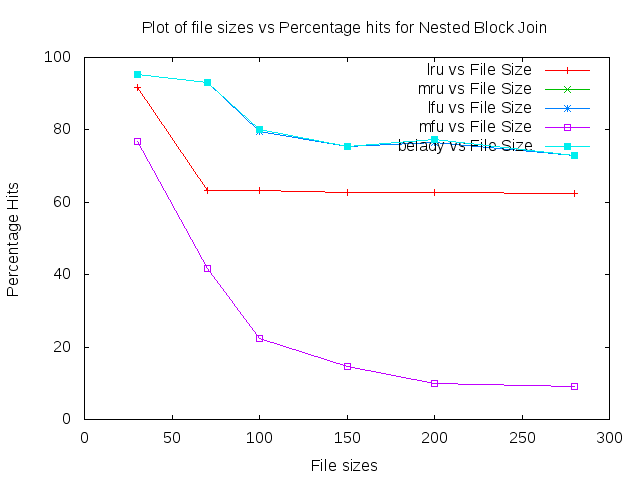
\includegraphics[width=12cm, height=9cm]{nestedblockjoinfilesize.png}

\end{figure}
\begin{figure}[H]
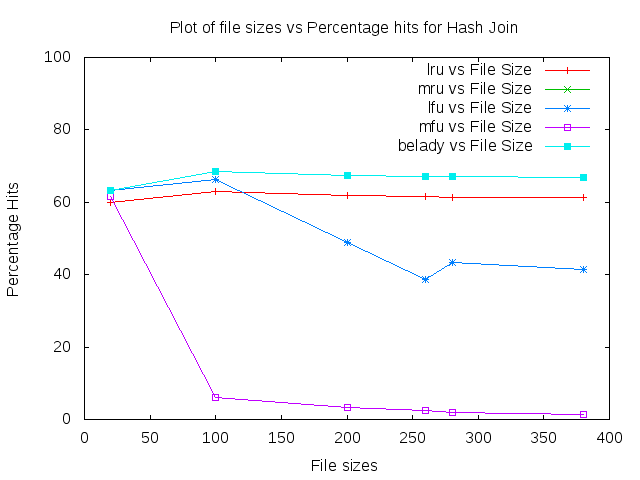
\includegraphics[width=12cm, height=9cm]{hashjoinfilesize.png}

\end{figure}
\begin{figure}[H]
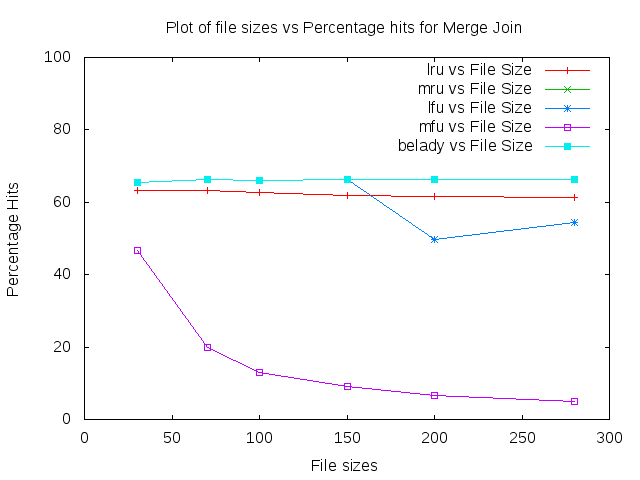
\includegraphics[width=12cm, height=9cm]{mergejoinfilesize.png}

\end{figure}
\begin{figure}[H]
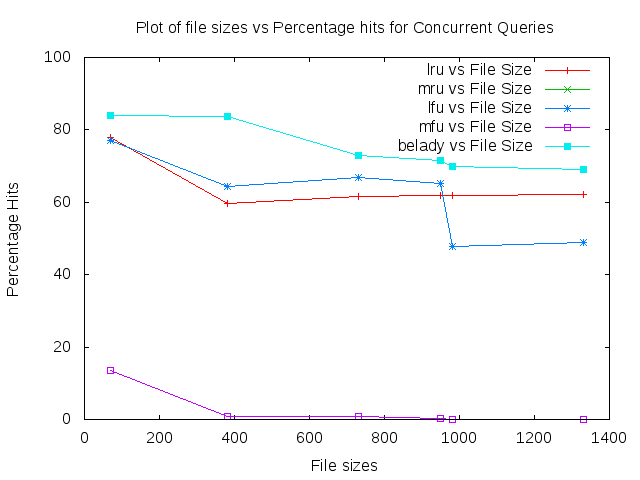
\includegraphics[width=12cm, height=9cm]{randomfilesize.png}

\end{figure}
\begin{figure}[H]
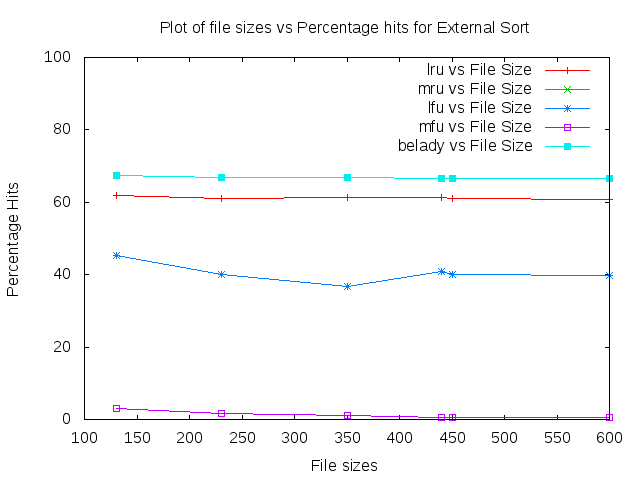
\includegraphics[width=12cm, height=9cm]{sortfilesize.png}

\end{figure}

\subsection*{{Inference}}

As we have seen that generally lru performs very good. But unlike the OS cache, this is not always the case. Infact many times other strategies perform better than lru. This is mainly because in case of databases when a particular operation is performed there is fixed access pattern like in nested block join we see that the block which was least recently used gets used again but lru removes it so gets a miss there. Similarly in case of other operations databases can have small predictability of the access pattern of access. And hence different techniques are employed at different points. The reasons for lru performing better in general is that in most cases when a block is too old is less likely to be used again. This is true for many operations. Thus is all these cases lru works very well. While in cases when there is round robin access the performance of lru degrades. This can be seen in the graphs as well. Thus we can infer that databases have to employ different strategy for different operations to get very high performance which is critical for the databases.


\section*{{Conclusion}}

We have simulated the buffer management strategies using the toydb which provides the low level code. We build on top of it. These strategies are back-bone of the buffer of any system. They can incur huge improvement in performance of the database. As it has been seen the graphs, there is a huge difference between the performance of various strategies. Thus we have learned about various aspects of buffer management and performance improvement on using the index. This gives huge information about internals of database systems which is crucial of designing large databases for real world application. Although toydb is simplistic but it has various features which is makes it good for the simulation and testing. In the end we have seen the lru performs very well in many cases but not in all. This shows that  buffer management for database is very different from the of OS where lru always works better. Thus buffer for database is different from that of OS and plays an important in database design.

\section*{{References}}
\begin{itemize}
\item Toydb source code
\item Toydb documentation
\item Gnuplot documentation
\item stackoverflow.org
\end{itemize}

\end{document}
